\documentclass{article}
\usepackage{amssymb, amsmath, amsthm}
\usepackage[margin=1in]{geometry}
\usepackage{verbatim}
\usepackage{graphicx}
\usepackage{hyperref} % \url \href

\newtheorem{definition}{Definition}
\newtheorem{theorem}{Theorem}
\DeclareMathOperator{\spn}{Span}

\usepackage[style=chem-acs ,backend=bibtex, sorting=none]{biblatex}
\addbibresource{ref_AutomaticTB.bib}

\begin{document}

\title{Molecular orbitals and symmetrization}
\author{Wenhao Zhang}
\date{\today}
\maketitle

\section{Introduction}

It is inefficient to learn rules using try and error, while the rules can be 
simply stated. 
Similarly, if we want to achieve the best results using machine learning, which 
basically learn from statistic distribution of data, 
it is important that we include as much concrete rules as possible,
which should greatly improve the accuracy of ML prediction while simplify the 
problems for ML so that fewer data are necessary.

To let machines predict the energy levels of the electronic states of moleculars, for example,
one way is to input the molecular structure to ML and ask it to output the energies. 
However, this naive approach suffer from the problems that 1) this `ab-initio' approach
is too complicated to be formulated as a simple function that we can understand 
and 2) if we ourselves cannot understand it, it is more difficult for us to inspect the 
machine learning output: Is machine really learning anything important, or it just 
found some other patterns that fits the data but does not agree with our physical 
or chemical understanding?

Using results from group theory, it is possible to simplify the Hamiltonians of 
a molecular systems. Such approach utilize symmetry and provide
rules that quantum mechanical interactions have to obey. 
In the simplest case, a $s$ type wavefunction can not interact with a $p$ type wavefunction on the 
same atom, because their intergrals are strictly zero. 
Furthermore, group theory analysis force the degeneracy of the energy levels.
These informations reduce the size of the problem considerably. As a consequence, to 
find the energy of the states, we now only need to consider the remaining interactions 
that are allowed between MOs, and the problem is then largely 
an electro-static one, which should be simple enough for machine learning to solve.
We try to formulate the ideas in the following sections

\section{Tight-binding Method}
\subsection{Tight-binding approximation}
Tight-binding methods is a well known technique to solve the band structure of 
crystalline material with a model Hamiltonian\cite{ziman_principles_1999}. 
It is fast to run and is able to 
reproduce the DFT calculated band structure accurately provided a suitable set of 
parameters. 
In the tight binding approximation, we write the Hamiltonian in the local 
basis orbitals:
\begin{equation}
    H_{ij}(R) = \langle \phi_{R',i} | H | \phi_{R'+R,j} \rangle = \langle \phi_{0,i} | H | \phi_{R,j} \rangle
\end{equation}
where index 0, $R$ refer to an arbitrarily selected `home' unitcell and unit cell at 
lattice vector $R$. The Bloch-like basis functions are then:
\begin{equation}
    |\psi_j^k\rangle = \sum_R e^{ik\cdot(R+t_j)} |\phi_{Rj} \rangle
\end{equation}
and the Hamiltonian matrix at reciprocal vector $\mathbf{k}$ is related to the 
Hamiltonian in real space by:
\begin{equation}
    H_{ij}^{\mathbf{k}} = \langle \psi_i^k | H |\psi_j^k\rangle = \sum_R e^{ik\cdot(R+t_j-t_i)} = H_{ij}(R)
\end{equation}
Diagonalizing the square matrix $H_{ij}^{\mathbf{k}}$ gives the eigen energies at $\mathbf{k}$
in the tight-binding approximation. 

\subsection{Solving the density of states}
Given a tight-binding model, the electronic density of states can be found by solving the 
Hamiltonian on a regularly spaced $\mathbf{k}$-grid, and straightforwardly calculated 
by numerical intergration methods, such as a summation of Gaussian peaks or tetrahedron methods. 

\section{Method}
\subsection{Work flow}
Our work concern the learning of a tight-binding approximation of crystalline materials 
with atomic orbitals as basis functions. The key approximation in this work is the 
nearest neighbor interaction approximation for the tight-binding interaction matrix elements. 
Furthermore, symmetry relationship is used to reduce the number of tight-binding parameters.
After obtaining the tight-binding model, the approximate band structure can be calculated 
by diagonalizing the Hamiltonian at the given $\mathbf{k}$ point. 

The overall workflow of our work is as follows in Figure \ref{F:forward_workflow}.
\begin{figure}[h]
    \centering
    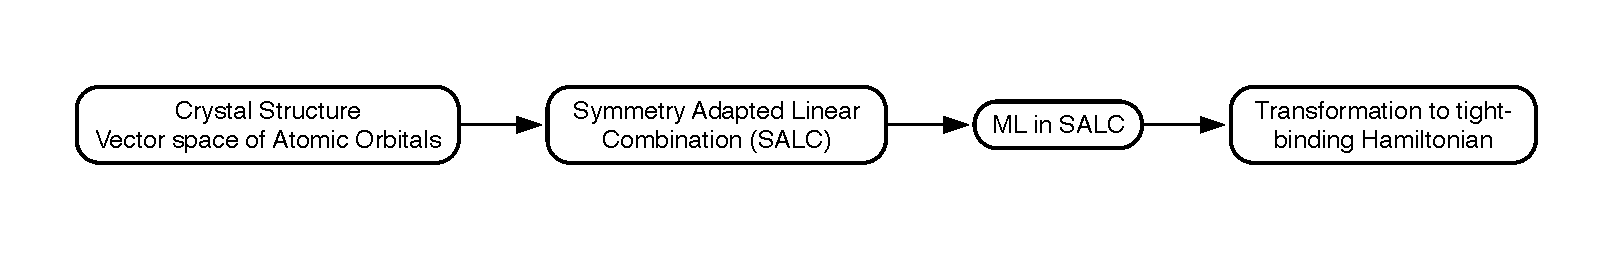
\includegraphics[width=5in]{figures/forward_workflow.pdf}
    \caption{Prediciton work flow of the tight-binding model generation process}
    \label{F:forward_workflow}
\end{figure}
For an atom $i$ in the input structure and a given set of atomic orbitals on $i$ and its neighbors as basis functions, 
we first identify site symmetry of this cluster and find the symmetry adapted linear combination as molecular orbitals (MO) basis 
functions corresponding to different representations. If two MOs belong to different irreducible representation, we simply 
set their interaction to be zero, otherwise, we use ML to predict their matrix elements. 
From the interactions in MO basis functions, we can apply transformation from MO to AO again, which yield the tight-binding 
Hamiltonian in atomic orbital basis functions.
Detailed treatment are presented in the following sections. 

\subsection{Symmetry adapted linear combinations}
According to the result from application of group theory in quantum chemistry, it can be 
shown that the eigenfunction of the Hamiltonian occupy differrent subgroups, each 
corresponding to a representation of the group of symmetry operation. Given a set of 
functions, the vector space span by them can be written as a direct sum of these 
\emph{invariant subspace}, and we can project any arbitrary functions into different 
components corresponding to these representations. This procedure is based on characters 
of the group representations and the orthogonal theorem for characters\cite{dresselhaus_group_2008}. 
For a detailed treatment and introduction to the method, see Appendix A.

Let's consider the example of group $D_{3h}$ corresponding to a molecular with one atom sitting 
on the origin and three atoms sitting on each tip of triangle lying in the $xy$ plane. We consider 
the three dimensional vector space span by three $s$ functions on each of the three atoms:
\begin{equation}
    V = \spn(|s_1\rangle, |s_2\rangle, |s_3\rangle)
\end{equation}
The projection operator into each invariant subspace of the representation $\Gamma_i$ is given by:
\begin{equation}
    P^{\Gamma_i} = \frac{l_i}{h} \sum_R \chi^{\Gamma_i}(R) P_R
\end{equation}
where $l_i$ is the dimension of the representation, $h$ is the order of the group, 
$\chi^{\Gamma_i}(R)$ is the character of the symmetry operation $R$ in this representation 
and $P_R$ is the symmetry operator in the basis of $|s_1\rangle, |s_2\rangle, |s_3\rangle$. 
Applying the projection operator onto each basis function, for all the representation, 
gives the result:
\begin{equation}
    | \psi^{A_1'} \rangle = P^{A_1'}|s_1\rangle = P^{A_1'}|s_2\rangle = P^{A_1'}|s_3\rangle 
    = \frac{\sqrt{3}}{3} (|s_1\rangle + |s_2\rangle + |s_3\rangle)
\end{equation}
which give the basis vector for the one dimensional subspace of representation $A_1'$, 
we also have:
\begin{align}
    |\psi_1^{E'}\rangle &= P^{E'} | s_1 \rangle = \frac{\sqrt{6}}{6}(\ \ \ 2|s_1\rangle - |s_2\rangle - |s_3\rangle) \\
    |\psi_2^{E'}\rangle &= P^{E'} | s_2 \rangle = \frac{\sqrt{6}}{6}(- |s_1\rangle + 2|s_2\rangle - |s_3\rangle) \\
    |\psi_3^{E'}\rangle &= P^{E'} | s_3 \rangle = \frac{\sqrt{6}}{6}(- |s_1\rangle - |s_2\rangle + 2 |s_3\rangle) \\
\end{align}
for the two dimension representation $E'$, where we find $|\psi_3^{E'}\rangle = - (|\psi_1^{E'}\rangle + |\psi_2^{E'}\rangle)$
showing that the three function projected indeed form a two dimensional subspace. 

After separating the invariant subspaces into different irreducible representations, the problem remains to 
find the suitable basis functions. 
To do so, we use the fact that a irreducible representation become 
reducible when the number of symmetric decreases. 
The functions belong to the irreducible representation of the symmetry group will split into different 
irreducible representation of the subgroup, each exhibit symmetry properties with respect to the reminding 
symmetry operations. 

As an example, in $D_{3h}$, any function in the subspace $E'$ can be written as a linear combination
of two of the three projected functions $|\psi_1^{E'}\rangle$, $|\psi_2^{E'}\rangle$ and $|\psi_3^{E'}\rangle$. 
By descending down symmetry to group $C_s$, which is a subgroup 
of $D_{3h}$ with only two elements: $\{E, \sigma_v\}$ where $\sigma_v$ is one of the three vertical reflection, 
choosen arbitrarily, $E'$ splits into two one dimensional representation $A'_{C_s}$ and $A''_{C_s}$.
Projection of the three functions in $E'$ with character table of $C_s$ yield 
one basis function for each one-dimensional representation:
\begin{align}
    |\psi^{E'\to A'} \rangle &= \frac{2}{\sqrt{6}} |s,2\rangle - \frac{1}{\sqrt{6}} |s,1\rangle - \frac{1}{\sqrt{6}} |s,3\rangle \\
    |\psi^{E'\to A''}\rangle &= \frac{\sqrt{2}}{2} |s,1\rangle - \frac{\sqrt{2}}{2} |s,3\rangle
\end{align}
Being the one dimensional representation of $C_s$, we can identify them to be 
symmetric and anti-symmetric under vertical mirror reflection. 

\subsection{Symmetry Adapted Tight-binding methods}
To simplify the machine learning problem, we focus on reducing the number of parameters 
in the tight-binding model that machine learning method need to predict. First, we utilize 
the fact that the interaction between atomic orbitals basis functions decay fast 
in real space. In the simplest case, only nearest neighbor interaction can be considered. 
Suppose that the average number of neighbors is $N_n$ and we have $N_{ao}$ basis functions 
on each atom, we would have:
\begin{equation}
    \text{Number of interaction} = ( N_n + 1 ) N_{ao}^2 / 2
\end{equation}
where division by $2$ remove the double counting (assuming the Hamiltonian is real, and 
therefore $\langle \phi_1 | H | \phi_2 \rangle = \langle \phi_2 | H | \phi_1 \rangle$). 

On the other hand, a tight-binding model with the nearest neighbor interaction can be further 
simplified using the result from symmetry analysis, and it turns out that 
symmetry restrict the value of and relationship between the matrix elements. 
The key point here is to consider the interaction in terms of MOs.
To illustrate the idea, we use the above example of a molecular in $D_{3h}$ symmetry and 
study the tight-binding parameter between the $|s\rangle$ on $|p_x\rangle$, $|p_y\rangle$
and $|p_z\rangle$ orbital on the origin. 
The three $p$ oribtal can be classified to be of representation 
$|p_z\rangle: A'$, 
$|p_x\rangle: E'\to A'$ and 
$|p_y\rangle: A'\to A''$. 

Since bonding can only be non-zero between vectors in the same representation, for $p_z$ we have
the following linear equation
\begin{align*}
    \frac{\sqrt{3}}{3} (\langle p_z | H | s_1 \rangle + \langle p_z | H | s_2 \rangle + \langle p_z | H | s_3 \rangle) = A \\
    \frac{\sqrt{6}}{6} (2\langle p_z | H | s_2 \rangle - \langle p_z | H | s_1 \rangle - \langle p_z | H | s_3 \rangle) = 0 \\
    \frac{\sqrt{2}}{2} ( \langle p_z | H | s_1 \rangle - \langle p_z | H | s_2 \rangle) = 0
\end{align*}
where $A$ stand for some arbitrary parameter. Solving this linear 
equation give the result:
\begin{equation}
    \langle p_z | H | s_1 \rangle = \langle p_z | H | s_2 \rangle = \langle p_z | H | s_3 \rangle = a
\end{equation}
which agrees with the symmetry relationship between the orbits.
Similarly, for $p_x$ and $p_y$ orbital and let $s_2$ on the $x$ axis. we can find:
\begin{gather}
    2 \langle p_x | H | s_1 \rangle = - \langle p_x | H | s_2 \rangle = 2 \langle p_x | H | s_3 \rangle = b \\
    \langle p_y | H | s_2 \rangle = 0;\quad \langle p_y | H | s_1 \rangle = - \langle p_y | H | s_1 \rangle = c
\end{gather}
so that only three parameter is required to describe nearest neighbor tight binding interaction between the 
$p$ orbitals at the center and the $s_i$ for $i = 1,2,3$:
\begin{table}[h]
    \caption{Interaction matrix elements}
    \label{T:interaction_D_3h}
    \centering
    \begin{tabular}{|c|ccc|}
        \hline
        $\langle \psi_1 | H | \psi_2 \rangle$ & $s_1$ & $s_2$ & $s_3$ \\ \hline
        $p_x$ & $b/2$ & $-b$ & $b/2$ \\
        $p_y$ & $c$ & $0$ & $-c$\\
        $p_z$ & $a$ & $a$ & $a$ \\
        \hline
    \end{tabular}
\end{table}


\subsection{Machine learning Matrix elements}

\newpage

\subsection{Deep Tensor Neural Network (DTNN)}
To utilize the symmetry relationship in the first way, we use the equivariant neural network
structure purposed by Thomas et al.\cite{thomas_tensor_2018} (Deep Tensor Neural Network). 
The network structure (DTNN) is reviewed in Appendix B. 
An important point that separate the equivariant network with general networks using 
invariant descriptors is that the transformation properties are kept in all layers of the equivariant
network such as one purposed by Thomas et al, but transformation properties are not kept if we 
use invariant descriptors. For example, the output of DTNN will change sign for a scalar output  
if a $\pi$ rotation is applied to an $p$ orbital, while the output will be the same for any
simple invariant network. This is one of the key property that we desire.
Furthermore, data in DTNN naturally flow in the form of tensor, which allow us to define 
tensor product, as in the case of Hamiltonian.

\subsection{Using the equivariant network}
Our network take inputs as two vectors and produce a scalar number. Since DTNN's output is 
also vector quantity, we define the network as $H(i,j)$ that operate on vector $| \psi_j \rangle$
\begin{equation}
    H |\psi\rangle = H(| \psi_i \rangle,| \psi_j \rangle) | \psi_j \rangle
\end{equation}
so that the tight-binding matrix element is naturally:
\begin{equation}
    H_{ij} = \langle \psi_i | H | \psi_j \rangle
\end{equation}
DTNN is rotational equivariant, meaning that we have: $H R | \psi_j \rangle  = RH | \psi_j \rangle $, 
as in a general equivariant network, 
where $R$ is an symmetry operation. 

let's now we consider how to use the above result to reduce the number of 
tight-binding matrix element to learn. 
We focus on nearest neighbor interaction and consider the above example, where
we place $p_x$ orbital at the center and two $s^1$, $s^2$ orbitals at $r_1 = (1,0,0)$ and $r_2 = (-1,0,0)$. 
How $s^1$ transform to $s^2$ is not unique, but we consider a $C_2$ rotation for concreteness. 
However, we do not include translation in our consideration but only the point group 
operations (vector transformation). 

Knowing the energy $\langle p_x | H | s^1 \rangle$, how do we derive the energy 
of $\langle p_x | H | s^2 \rangle$? Since $| s^2 \rangle = R | s^1 \rangle$ We have:
\begin{equation}
    \langle p_x | H | s^2 \rangle = \langle p_x | H R | s^1 \rangle
    = \langle p_x | R H | s^1 \rangle = \langle R^{-1} p_x | H | s^1 \rangle
\end{equation}
Since we know how rotation transform $p_x$, we recover the relationship 
\begin{equation}
    \langle p_x | H | s^2 \rangle = - \langle p_x | H | s^1 \rangle
\end{equation}

As a second example, let's consider $pp_{\sigma}$ bond, replacing $s^1$ with $p_x^1$ 
and $s^2$ with $-p_x^2$. Note the negative sign ensures that two orbitals at $r_1$ and $r_2$
are generated by point group symmetry. 
We have:
\begin{equation}
    - \langle p_x^0 | H | p_x^2 \rangle =  - \langle p_x^0 | HR | p_x^1 \rangle 
    = - \langle p_x^0 | RH | p_x^1 \rangle = \langle p_x^0 | H | p_x^1 \rangle
\end{equation} 
which is again the correct results. 



\newpage
\appendix

\section{Character table for site symmetry groups}
\subsection{Finding the character}
In this section, we discuss the procedure to find the characters for the 
symmetry operations in the site symmetry of each atoms. For crystals with 
symmetry group $G$ and a point $\mathbf{x}$, the subgroup of $G$ that leave
the given point fixed is called the \emph{site symmetry groups} $S_{\mathbf{x}}$ of that point. 
Writing a space group operation as matrix--column pair $(\mathbf{W},\mathbf{w})$, 
it is straightforwardly to see that for group elements in $S_{\mathbf{x}}$ 
contain no translation. 

In crystals, the number of possible site symmetry is greatly reduced compared to 
that in the moleculars. Possible rotations can be characterized by the trace 
and determinant of the rotation matrix, where the $\det\mathbf{W}$ indicate the 
existance of inversion in the operation and $\text{tr}\mathbf{W}$ gives the angle of rotation. 
Since trace is invariant under permutation, angle of rotation does not depend on the 
basis vector of the symmetry matrix. The characterization is listed by table \ref{T:operation_properties}.
\begin{table}[h]
    \centering
    \caption{Site symmetry types}
    \begin{tabular}{|c|cccccccccc|}
        \hline
        $\det$      & +1 & +1 & +1 & +1 & +1 & -1 & -1 & -1 & -1 & -1 \\ 
        $\text{tr}$ &  3 &  2 &  1 &  0 & -1 & -3 & -2 & -1 &  0 &  1 \\  
        \hline
        type        &  1 &  6 &  4 &  3 &  2 & -1 & -6 & -4 & -3 & -2 = m \\ 
        \hline
    \end{tabular}
    \label{T:operation_properties}
\end{table}

The total number of crystallographic point groups in three dimension is 32, and their character tables are 
tabulated either in The point group table of the bilbao crystallographic server \href{https://www.cryst.ehu.es/rep/point.html}{bilbao}. 
In crystallographic server, all the matrix element of the operations are also given explicitly, in the respective basis vector 
and denoted in Seitz symbol. Their characters can also be found from the same webpage.
Seitz symbols are tabulated as well (Seitz symbols for crystallographic symmetry operations)
with the standard basis vectors given in the international table for each crystal system. 
In our implementation, the character table of the 32 point symmetry groups are taken from bilbao server and 
stored. For hexagonal lattice, we use the hexagonal setting.

However, one complication arise when the site symmetry operation does not correspond to the standard basis. For example, 
in a cubic crystal belong to space group $Pm\bar{3}m$ (221), the point $(x,x,x)$ on the body diagonal has site symmetry $3m$
whose rotation matrix is tabulated in hexagonal basis. Therefore, we cannot directly compare the rotation matrix of the 
site symmetry operation with the ones tabulated in the Bilbao server. Instead, we use the following method to generate 
the seitz symbol from a list of rotation matrices, and then use the seitz symbol to assign characters to each symmetry 
operations. The input rotation matrices can correspond to any orientation.

A seitz symbol consist of three parts: type of the symmetry operation, sense of the rotation 
(for rotation $4$, $-4$, $3$, $-3$, $6$, $-6$ only) and the characteristic direction. 
Symmetry type can be found according to table \ref{T:operation_properties}. To find the 
symmetry direction in the standard basis, we first find the symmetry direction in the cartesian coordinate. 

For symmetry $1$ or $\bar{1}$, a point $(0.0, 0.0, 0.0)$ will be assigned. If the symmetry operation is a rotoinversion,
we multiplicity it by $-\mathbf{1}$ to obtain the rotation parts $\mathbf{W}$. 
The symmetry direction is given by finding the eigenvector with eigenvalue $1$. 
\begin{equation}
    \label{E:rotation_axes}
    \mathbf{W}\mathbf{v} = \mathbf{v}
\end{equation}

After computing the directions of all the symmetry operation, we separate them into sets that are related by symmetry operations:
\begin{equation}
    \{\mathbf{v}' \mid \mathbf{W}\mathbf{v}, \mathbf{W} \in \mathbf{R}\}
\end{equation}
All symmetry direction belonging to the same set contain the same symmetry elements, and they correspond to the symmetry directions 
used in Hermann--Mauguin symbol. For example, the result of the classification is listed in table \ref{T:6mmm} for group $6/mmm$
\begin{table}[h]
    \centering
    \caption{Symmetry operation and directions in cartesian coordinate in $6/mmm$}
    \begin{tabular}{|c|l|l|}
        \hline
        Operation & Directions & Symmetry Direction\\
        \hline
        -1,1 & (  0.0  0.0  0.0) & $\mathbf{0}$\\
        6,-3,-6,m,2,3 & (  0.0  0.0  1.0) & $[001]$\\
        m,2 & (-0.5,-0.866,0.0), (1.0,0.0,0.0), (-0.5,0.866,0.0) & $[100],[010],[\bar{1}\bar{1}0]$\\
        m,2 & (0.866,-0.5,0.0), (0.0,1.0,0.0), (-0.866,-0.5,0.0) & $[120],[\bar{2}\bar{1}0],[1\bar{1}0]$\\
        \hline
    \end{tabular}
    \label{T:6mmm}
\end{table}

Then, it is possible to choose the basis for the site symmetry group. The choice of 
the axes are listed in table \ref{T:choice_of_axes}. 
After choosing $\mathbf{a}$ and $\mathbf{b}$, $\mathbf{c}$ is chosen so that the three axes
form a right-handed system: $(\mathbf{a}\times \mathbf{b}) \cdot \mathbf{c} > 0$. 
The direction in cartesian coordinates corresponding to the symmetry direction in the seitz symbol can also be computed and can be 
compared to the symmetry direction found using equation \eqref{E:rotation_axes}. Finally, the 
sense of the rotation can be computed using the method provided by 
\emph{Efficient conversion from rotating matrix to rotation axis and angle by extending Rodrigues’ formula},
by calculating the $\sin\theta$. 

\begin{table}[h]
    \centering
    \caption{Choice of $\mathbf{a}$, $\mathbf{b}$ and $\mathbf{c}$}
    \begin{tabular}{|c|c|}
        \hline
        Groups & Choice\\
        \hline
        \begin{tabular}{c}$2$, $m$, $2/m$, $4$, $-4$, $4/m$\\$3$, $-3$, $6$, $-6$, $6/m$\end{tabular}
            & $z = [001]$ \\ \hline
        $222$, $mm2$, $mmm$ & $x=[100],y=[010],z=[001]$ \\\hline
        $32$, $3m$, $-3m$, $622$, $6mm$, $-6m2$, $6/mmm$ & $\{x, y\} \in \{[100], [010],[\bar{1}\bar{1}0]\}$ \\\hline
        $23$, $m-3$, $432$, $-43m$, $m-3m$ & $\{x,y,z\} = \{[100],[010],[001]\}$ \\
        \hline
    \end{tabular}
    \label{T:choice_of_axes}
\end{table}

\subsection{Symmetry reduction}
In our application, we need to find the subgroup of the site symmetry group so that we can separate basis 
uniquely for a representation with more than one dimension. To do so, we need to know which symmetry is 
kept when we move from a group to its subgroup. Finding the subgroups is not a trivial task and we 
manually assign maps from the seitz symbol of the subgroup to the ones in the supergroup. In this way, subgroup
and the correspond characters are readily obtained onces the seitz symbol of the site-symmetry group is known.

\subsection{Subduction}
Subduction enable us to perform symmetry descend that split the irreducible representation into 
different subspaces with different symmetry. 

\section{Groups, representations and basis}
\subsection{Groups and representations}
The symmetry operation that map a molecular onto itself form a group $G$. From a group,
we define a representation of group $G$ as a mapping:
\begin{definition}
    A linear \emph{representation} of a group $G$ on a vector space $V$ is a homomorphism:
    \[\rho\colon G \to \text{GL}(V)\]
    where homomorphism is a mapping that satisfies $\rho(g_1g_2) = \rho(g_1)\rho(g_2)$.
\end{definition}
Representations are not unique: a change of basis leads to an equivalent representation 
and the direct sum of two representation is again a representation. However, representations
can be uniquely reduced to so called \emph{irreducible representations}.
We define the notion of \emph{invariant vector space}:
\begin{definition}
    For any vector $v$ in $V$, for any $g\in G$, if we have $\rho(g)v \in V$, then $V$
    is an invariant vector space.
\end{definition} 
For a representation with vector space $V$, $V$ is an invariant to the group $G$. 
If there exist a vector space $W\subset V$ which is also invariant to $G$, then we call $W$
an \emph{invariant subspace}. 
Furthermore, there exist another invariant subspace $U$ of $V$ so that $V$ is given by a direct sum:
\begin{equation}
    V = U \oplus W
\end{equation}
By splitting the vector space $V$ into invariant subspaces until it is not possible, we find the 
\emph{irreducible representation} by the reducible representation on $V$, and the matrix form 
of the reducible representation can be written as the block diagonal form
\begin{equation}
    \rho^{\Gamma}(g) = \left(  
        \begin{matrix}
            \rho^{\Gamma_1} (g) & 0 & \cdots\\
            0 & \rho^{\Gamma_2} (g) & \\
            \vdots &  & \ddots
        \end{matrix}
    \right)
\end{equation}
where $\Gamma$ denote the reducible representation and $\Gamma_i\ (i = 1, \dots)$ index 
the irreducible representations.

\subsection{Basis functions}
For each invariant subspaces corresponding to a representation $\Gamma_n$, we write its basis 
functions using the braket notation $|\Gamma_n,j\rangle$. For a irreducible representation with 
dimension $N$, we have $N$ such basis functions and any vectors in this invariant subspace 
can be written as a linear combination:
\begin{equation}
    |\phi^{\Gamma_n}\rangle = \sum_{i = 1}^N c_i |\Gamma_n,i\rangle
\end{equation} 
Due to the definition of invariant subspace, the matrix representation of $G$ in the invariant 
subspace will have the form:
\begin{equation}
    \rho^{\Gamma_n}(g)_{ij} = \langle \Gamma_n,i | P_g | \Gamma_n,j \rangle
\end{equation}
where $P_g$ is the symmetry operation. 
For reducible representations $\Gamma_{r}$, its vector subspace is a direct sum of all the subspace 
of irreducible representations it contains. Therefore, basis functions from irreducible 
subspaces together form the basis functions for the reducible representation.

The basis functions of the representation of the symmetry group is closely connected to quantum mechanics.
Since the Hamiltonian of the system is invariant to the symmetry operation, we have the commutation 
relationship:
\begin{equation}
    [P_g,H] = 0
\end{equation}
for any symmetry operation $g$. As a consequence, if $|\phi_{\varepsilon_i}\rangle$ an eigenfunction of $H$
with eigenvalue $\varepsilon_i$, $P_g|\phi_{\varepsilon_i}\rangle$ will also be an eigenfunction 
with degenerate eigenvalues. Since $|\phi_{\varepsilon_i}\rangle$ and $P_g|\phi_{\varepsilon_i}\rangle$
together will define some invariant space. Therefore, it is possible to classify the eigenfunctions of the 
Hamiltonian according to the subspaces which they occupy, and the set of degenerate eigenfunctions are 
related by symmetry operation. 

\section{Finding the representations and Symmetry adopted basis functions}
\subsection{Molecular orbitals}
Using character table and the orthogonality theorem for characters, we can find the basis functions 
of the Hamiltonians knowing only the symmetry property of the structure. 
We start by finding the vector space of all the participating atomic orbitals and their transformation 
properties under group operation, then decompose the reducible representation to irreducible ones. 
We follow the example of Dresselhaus\cite{dresselhaus_group_2008} and consider the group $D_{3h}$ with 
the following character table \ref{T:ct}
\begin{table}[h!]
    \centering
    \caption{Character table of $D_{3h}$}
    \begin{tabular}{|c|c|c|c|c|c|c|}
                & $E$ & $\sigma_h$ & 2$C_3$ & 2$S_3$ & 2$C_2'$ & 3$\sigma_v$ \\ \hline
         $A_1'$ &  1  &  1         &  1     &  1     &   1     &   1         \\
         $A_2'$ &  1  &  1         &  1     &  1     &  -1     &  -1         \\
         $A_1''$&  1  & -1         &  1     & -1     &   1     &  -1         \\
         $A_2''$&  1  & -1         &  1     & -1     &  -1     &   1         \\
         $E'$   &  2  &  2         &  -1    & -1     &   0     &   0         \\
         $E''$  &  2  & -2         &  -1    &  1     &   0     &   0         \\ \hline
    \end{tabular}
    \label{T:ct}
\end{table}
Suppose we have four atoms, one on the rotation axis and three other that transform to each other 
by three fold rotation, and $s$ and $p$ orbitals on each of the atoms. Indexing each atomic 
centered functions using atomic index $i$ and orbital index $l,m$ as $| i,l,m \rangle$ 
(or $| i,s \rangle, \dots, |i,p_x\rangle$ if convenient), we form 
a vector space with dimension $4\times4 = 16$:
\begin{equation}
    V = \spn(| 1,s \rangle, | 1,p_x \rangle ,\dots, | 4,p_y \rangle, | 4,p_z \rangle)
\end{equation}
We can find the matrix elements of the symmetry group in this space using the following equation:
\begin{equation}
    \rho(g)_{ij} = \langle i | P_g | j \rangle
\end{equation}
where $\rho(g)$ is the matrix in the vector space of atomic basis function and $P_g$ is the 
operators that transform the basis functions. 
After generating the matrix of each symmetry operation, we find the character of the representation
in this atomic orbital basis:
\begin{gather*}
    \chi^{AOs}(E) = 16,\ \chi^{AOs}(\sigma_h) = 8,\ \chi^{AOs}(C_3) = 1\\ 
    \chi^{AOs}(S_3) = -1,\ \chi^{AOs}(C_2') = 0,\ \chi^{AOs}(\sigma_v) = 4
\end{gather*}
The uniqe decomposition of the reducible representation into the irreducible ones are given by:
\begin{gather}
    \chi(C_k) = \sum_{\Gamma_i} a_i \chi^{\Gamma_i}(C_k) \\
    a_i = \frac{1}{h} \sum_{k} N_k \chi^{\Gamma_i}(C_k)^* \chi(C_k)
\end{gather}
where $C_k$ and $N_k$ denote the class of symmetry operation (whose elements have the same character)
and their multiplicity. $h = |G|$ is the order of the group. Decomposing the 
above represention in atomic orbital space, we obtain the following relationship:
\begin{equation}
    \Gamma^{AOs} = 
      3\Gamma^{A_1'} + \Gamma^{A_2'}  + 2\Gamma^{A_2''} + 4\Gamma^{E'} + \Gamma^{E''}
\end{equation}

\subsection{Projecting into invariant subspace}
Knowing who the vector space constructed from the atomic orbitals can be organized into invariant subspaces 
under symmetry group does not tell us what these subspaces are. 
More importantly, to start to reason about the energy of these orbitals, we should start from the approximate
shape of these orbitals.

To start, we first identify what these subspaces are using the projection operation on the atomic basis functions
\begin{equation}
    P^{\Gamma_i} = \frac{l_n}{h}\sum_R \chi^{\Gamma_i}(R) P_R
\end{equation}
where $P^{\Gamma_i}$ is the projection operation onto the representation $\Gamma_i$, $l_n$ is the dimension of the 
representation. 
Operating this projection operator on an arbitrary function in the vector space $V^{AOs}$ produce a vector in the 
subspace that correspond to the required representation. In our previous example, 
if we consider the vector subspace formed by the $s$ orbital centered on three equivalent atoms corresponding to the 
corner of the triangle, the group representation can be decomposed to $\Gamma^{s3} = \Gamma^{A_1'} + \Gamma^{E'}$
with dimension one and two. 
Projecting from each of the $s$ function onto these subspaces, we find that, for $A_1'$:
\begin{align}
    \psi_1^{A_1'} = \frac{1}{3}|s,1\rangle + \frac{1}{3}|s,2\rangle + \frac{1}{3}|s,3\rangle 
    = \psi_2^{A_1'} = \psi_3^{A_1'}
\end{align}
i.e., the projectioned functions span a one dimensional subspace. 
For $E'$ which is a two dimensional subspace, projection gives:
\begin{align}
    \psi_1^{E'} &= \ \ \ \frac{2}{3}|s,1\rangle - \frac{1}{3}|s,2\rangle - \frac{1}{3}|s,3\rangle  \\
    \psi_2^{E'} &= -\frac{1}{3}|s,1\rangle + \frac{2}{3}|s,2\rangle - \frac{1}{3}|s,3\rangle  \\
    \psi_3^{E'} &= -\frac{1}{3}|s,1\rangle - \frac{1}{3}|s,2\rangle + \frac{2}{3}|s,3\rangle 
\end{align}
Noting that $\psi_3^{E'} = - (\psi_1^{E'} + \psi_2^{E'})$, we find that this is indeed a two dimension 
subspace. 

\subsection{Symmetry adopted linear combination}
After separating the invariant subspaces into different irreducible representations, the problem remains to 
find the suitable basis functions. These basis functions should be mutually orthogonality and, at the same times,
exhibit symmetry properties of the group. 
To do so, we need to reduce the symmetry of the system artifically. An irreducible representation become 
reducible when the number of symmetric decreases and the resulting subspaces will be linearly independent 
regarding to the subgroup. As an example, consider the above invariant subspace span by the three functions
$\psi_1^{E'}$, $\psi_1^{E'}$ and $\psi_1^{E'}$. It is clear that these three functions are related to each 
other by rotations, however, they are not orthogonal and each of them do not exhibit clear symmetry property
by themselves. Furthermore, the dimension of this subspace is two and we should eliminate one of the function
from these three, which cannot be done uniquely. 

By descending down symmetry, however, we are able to find better basis functions: group $C_s$ is a subgroup 
of $D_3h$ with only two elements: $\{E, \sigma_v\}$ where $\sigma_v$ is one of the three vertical reflection, 
choosen arbitrarily. 
The two dimensional representation $E'$ splits under the reduction of symmetry into two one dimensional representation.
Projection of the three functions in $E'$ yield one basis function for each one dimensional representation:
\begin{align}
    \psi_1^{A'} &= \frac{2}{\sqrt{6}} |s,2\rangle - \frac{1}{\sqrt{6}} |s,1\rangle - \frac{1}{\sqrt{6}} |s,3\rangle \\
    \psi_1^{A"} &= \frac{\sqrt{2}}{2} |s,1\rangle - \frac{\sqrt{2}}{2} |s,3\rangle
\end{align}
Being the one dimensional representation of $C_s$, we can identify them to be 
symmetric and anti-symmetric under vertical mirror reflection. 

\section{Euclidean neural network}
\subsection{Euclidean neural network}

Euclidean nueral network purposed by Thomas et al. 2018\cite{thomas_tensor_2018} is different from the previous network in that
\emph{The euclidean neural network operate on points throughout the structure: convolution is performed on each point with respect to other points.}
Equivariance is achieved by their definition of point convoultion, but is simpler in the form because the discreteness of the 
points.

At each layer, each point $a$ in the point cloud are associated with a vector $(\mathbf{r}_a, \mathbf{x}_a)$ 
in the vector space $R^3 \oplus \mathcal{X}$, where $\oplus$ indicate direct sum. We require that vector space $\mathcal{X}$ are span 
by the spherical harmonics $Y_m^l$ for $0\leq l \leq b$ and $|m|\leq l$. We denote such a feature 
vector as $V_acm^l$, where $c$ denotes channels (depth). 
Under a rotation $R$ around a chosen origin, The input feature thus transforms as:
\begin{equation}
    (\mathbf{r}_{a}, V_{acm}^l) \to (R \mathbf{r}_{a}, \sum_{m'}D_{mm'}^l(R)V_{acm'}^l) \label{E:3dnn_rotation_input}
\end{equation}

We define a filter to be of the following form:
\begin{equation}
    F_{cm_f}^{l_f, l_i}(\mathbf{r}) =  R_c^{l_f, l_i} (r) Y_{m_f}^{l_f}(\mathbf{r})
\end{equation}
with $r = |\mathbf{r}|$, and $R_c^{l_f, l_i} (r)$ are the parameter of the filter function that can be learned.
The filter functions are equivariant to rotation:
\begin{align}
    F_{cm_f}^{l_f, l_i}(R\mathbf{r}) &= R_c^{l_f, l_i} (r) Y_{m_f}^{l_f}(R\mathbf{r}) \\
    &= R_c^{l_f, l_i} (r) \sum_{m_f'} D_{m_fm_f'}^{l_f}(R)  Y_{m_f}^{l_f}(\mathbf{r})
\end{align}
In the following, we will first define the components of the network.
Then we will show that they are equivariant to rotation. As well as 
invariant to translation and permutation.

\subsection*{Point convolution}
we define a convolution layer as:
\begin{align}
    V_{acm_o}^{l_o} &= L^{l_o}_{acm_o} (\mathbf{r}, V_{cm_i}^{l_i}) \notag\\
    &= \sum_{m_f, m_i} C^{l_o,m_o}_{(l_f, m_f)(l_i,m_i)} \sum_{b \in S} F_{cm_f}^{l_f, l_i}(\mathbf{r}_{ab}) V^{l_i}_{bcm_i} \label{E:3dnn_point_convolution}
\end{align}
where $l_i$ and $l_f$ is the rotation order of the input and the filter, $m = -l_f, \dots, l_f$ is the index of the basis function.
$C^{l_o,m_o}_{(l_f, m_f)(l_i,m_i)}$ is the \emph{Clebsch-Gordan coefficients}
Note that we do not contain index $a$ in \[L^{l_o}_{acm_o} (\mathbf{r}, V_{cm_i}^{l_i})\] because
the output depend on the feature vector $(\mathbf{r}, V_{cm_i}^{l_i})$ from all points in the set $S$.
Note that we can understand the 'convolution' as the convolution between the filter function and a delta function 
marking the position of the point, at $\mathbf{r}_{ab}$.

Since the output only depend on relative distance $\mathbf{r}_{ab} = \mathbf{r}_{a} - \mathbf{r}_{b} $, 
the output is invariant under a translation of all points. Also, the summation in Equation \eqref{E:3dnn_point_convolution}
means the result is invariant under permutation of points.

We can show that the above point convolution is equivariant to rotation (Appendix \ref{A:proof_equivariance_point}):
rotation on the input feature space $(l_i,m_i)$ 
correspond to rotation on output feature space $(l_o,m_o)$.

\subsection*{Self-interaction}
We define a self-interaction between the feature at each point $a$ as:
\begin{equation}
    V_{acm}^{l} = \sum_{c'} W^{l}_{cc'} V_{ac'm}^{l} 
\end{equation}
Such operation is independent on permutation and translation. It is also equivariant to rotation:
\begin{align*}
    [ W \circ R ] (V_{acm}^l) &= \sum_{c'} W^{l}_{cc'} \sum_{m'}D_{mm'}^l(R)V_{acm'}^l \\
                &= \sum_{m'}D_{mm'}^l(R) \sum_{c'} W^{l}_{cc'}  V_{acm'}^l \\
                &= [ R \circ W ] (V_{acm}^l)
\end{align*}
However, it should be noted that the self-interaction coefficients $W$ are used for every $m$. 
If for different $m$ we have different weight, we than have:
\begin{align*}
    [ W \circ R ] (V_{acm}^l) &= \sum_{c'} W^{lm}_{cc'} \sum_{m'}D_{mm'}^l(R)V_{acm'}^l \\
                &= \sum_{m'}D_{mm'}^l(R) \sum_{c'} W^{lm}_{cc'}  V_{acm'}^l 
\end{align*}
which is different from $\sum_{c'} W^{lm'}_{cc'}  V_{acm'}^l$ by first applying self-interaction.

\subsection*{Nonlinearity}
For nonlinearity, we can use:
\begin{align*}
    &h^l (V_{ac}^0 + b_c^0) & &\text{for $l=0$} \\ 
    &h^l (\|V\|_{ac}^l + b_c^l)V_{acm}^{l} &  &\text{for $l>0$} \label{E:3dnn_nonlinearity}
\end{align*}
with $h\colon \mathbb{R}\to \mathbb{R}$ and 
\[ \|V\|_{ac}^l = \sqrt{\sum_m |V_{acm}^l|^2} \]
Nonlinearity is invariant for permutation and translation. For rotation, 
because rotation does not change length in the vector space, $\|V\|_{ac}^l$ is 
therefore invariant of rotation:
\begin{equation}
    \|D(R)V\| = \|V\|
\end{equation}
Thus, $h^l (\|V\|_{ac}^l + b_c^l)$ is invariant with respect to rotation. 
The rotational properties is the output is solely given by $V_{acm}^{l}$.
Therefore, nonlinearity defined by Equation \eqref{E:3dnn_nonlinearity} is equivariant
with respect to rotation.

\subsection*{Relationship with spherical CNNs}
Here, we show the euclidean neural network can be understood as a special case of the more general spherical CNNs 
with fixed filter.
We first consider Equation \eqref{E:3dnn_point_convolution} with $l_i=m_i=0$, i.e., only scalars on each point. 
Omitting the channel index $c$, 
equation \eqref{E:3dnn_point_convolution} becomes:
\begin{align}
    V_{am}^{l} &= \sum_{b \in S} F_{m}^{l}(\mathbf{r}_{ab}) V_{b}  \notag\\
            &= \sum_{b \in S} \left[R^{l} (|r|)V_{b}\right] Y_{m}^{l}(\mathbf{x})
\end{align}
The part in square bracket is scalar value. This activation can be achieved by convoluting a filter with
\begin{equation}
    f(\mathbf{r}) = \sum_{b \in S} \left[R^{l} (|r|)V_{b}\right] \delta(\mathbf{x}_{ab})
\end{equation}
$\delta(\mathbf{x}_{ab})$ is zero unless the projection of the point b fall on the sphere at $\mathbf{x}_{ab}$. 
We define the filter as:
\begin{equation}
    g_l(x) = \sum_{0\leq l \leq b} \sum_{|m|\leq l} Y_m^l(x)
\end{equation}
Putting the above form into Equation \eqref{E:convolution_s2}:
\begin{align*}
    V_a (r) &= \int_{s^2} \sum_{b \in S} \left[R^{l} (|r|)V_{b}\right] \delta(\mathbf{x}_{ab}) \sum_{l,m} Y_m^l(r^{-1}x) dx \\
    &= \sum_{l,m} \sum_{b \in S} \left[R^{l} (|r|)V_{b}\right] Y_m^l(r^{-1}\mathbf{x}_{ab}) \\
    &= \sum_{l,m} \sum_{b \in S} \left[R^{l} (|r|)V_{b}\right] \sum_n D_{mn}^l(r^{-1}) Y_n^l(\mathbf{x}_{ab}) \\
    &= \sum_{l,m,n} D_{mn}^l(r^{-1}) \sum_{b \in S} \left[R^{l} (|r|)V_{b}\right] Y_n^l(\mathbf{x}_{ab})
\end{align*}
The coefficients \[V_{an}^l = \sum_{b \in S} \left[R^{l} (|r|)V_{b}\right] Y_n^l(\mathbf{x}_{ab})\] therefore uniquely define 
the feature map on $r$. It describes the local environment of the points equivariantly to rotation $r$.

If the point $b$ are associated with $l>0$, then we also need to take into account the rotational property of these points. This is 
achieved using the properties of Clebsch-Gordan coefficients, similar to the addition of angular moment in quantum mechanics.

\section{Tight-binding model in Halide Perovskite Semiconductors}
We describe the parameters in the cubic Halide Perovskite described in 
the work of Boyer et al.\cite{boyer-richard_symmetry-based_2016} as the 
our reference model. The parameters are as follows:
\begin{table}[h]
    \centering
    \caption{Tight binding parameters, Halide Perovskite Semiconductors}
    \label{T:TBP}
    \begin{tabular}{|c|c|c|}
        \hline
        Atom & Positions(crystal coord.) & Basis functions \\
        \hline
        B & $(0.0,0.0,0.0)$ & $|S_0\rangle$, $|X_0\rangle$, $|Y_0\rangle$, $|Z_0\rangle$ \\
        X & $(0.5,0.0,0.0)$ & $|S_1\rangle$, $|X_1\rangle$, $|Y_1\rangle$, $|Z_1\rangle$ \\
        X & $(0.0,0.5,0.0)$ & $|S_2\rangle$, $|X_2\rangle$, $|Y_2\rangle$, $|Z_2\rangle$ \\
        X & $(0.0,0.0,0.5)$ & $|S_3\rangle$, $|X_3\rangle$, $|Y_3\rangle$, $|Z_3\rangle$ \\
        \hline
    \end{tabular}
\end{table}
We have in total 16 atomic orbitals in the unit cell. In a $3\times 3\times 3$ supercell
which can include all the nearest neighbor interaction, We would have in total $N_s \times 16 \times 16$ parameters. 
Restricting the interaction to first order, only 304 interactions left. 
Now, we use the fact that orbitals belong to different symmetry cannot form bonding, 
so that matrix elements like $\langle S_0 | H | P_0 \rangle$ is zero, we can reduce the 
number of non-zero parameters. 
Finally, we use symmetry relationship to obtain relationship in bonding parameters. 
The interaction can be parameterized using only 9 parameters:
\begin{align*}
    E_{s0} &= \langle S_0 | H | S_0 \rangle \\
    E_{s1} &= \langle S_1 | H | S_1 \rangle \\
    E_{p0} &= \langle X_0 | H | X_0 \rangle \\
    E_{p1} &= \langle X_1 | H | X_1 \rangle 
\end{align*}
and 
\begin{align*}
    V_{ss} &= \langle S_0 | H | S_1 \rangle  \\
    V_{s0p1} &= \langle S_0 | H | X_1 \rangle \\
    V_{p0s1} &= \langle X_0 | H | S_1 \rangle \\
    V_{pp\sigma} &= \langle X_0 | H | X_1 \rangle \\
    V_{pp\pi} &= \langle Y_0 | H | Y_1 \rangle \\
\end{align*}




\printbibliography[title={Reference}]
\end{document}
